\documentclass{standalone}
\usepackage{tikz}
\usetikzlibrary{patterns, positioning}


\begin{document}
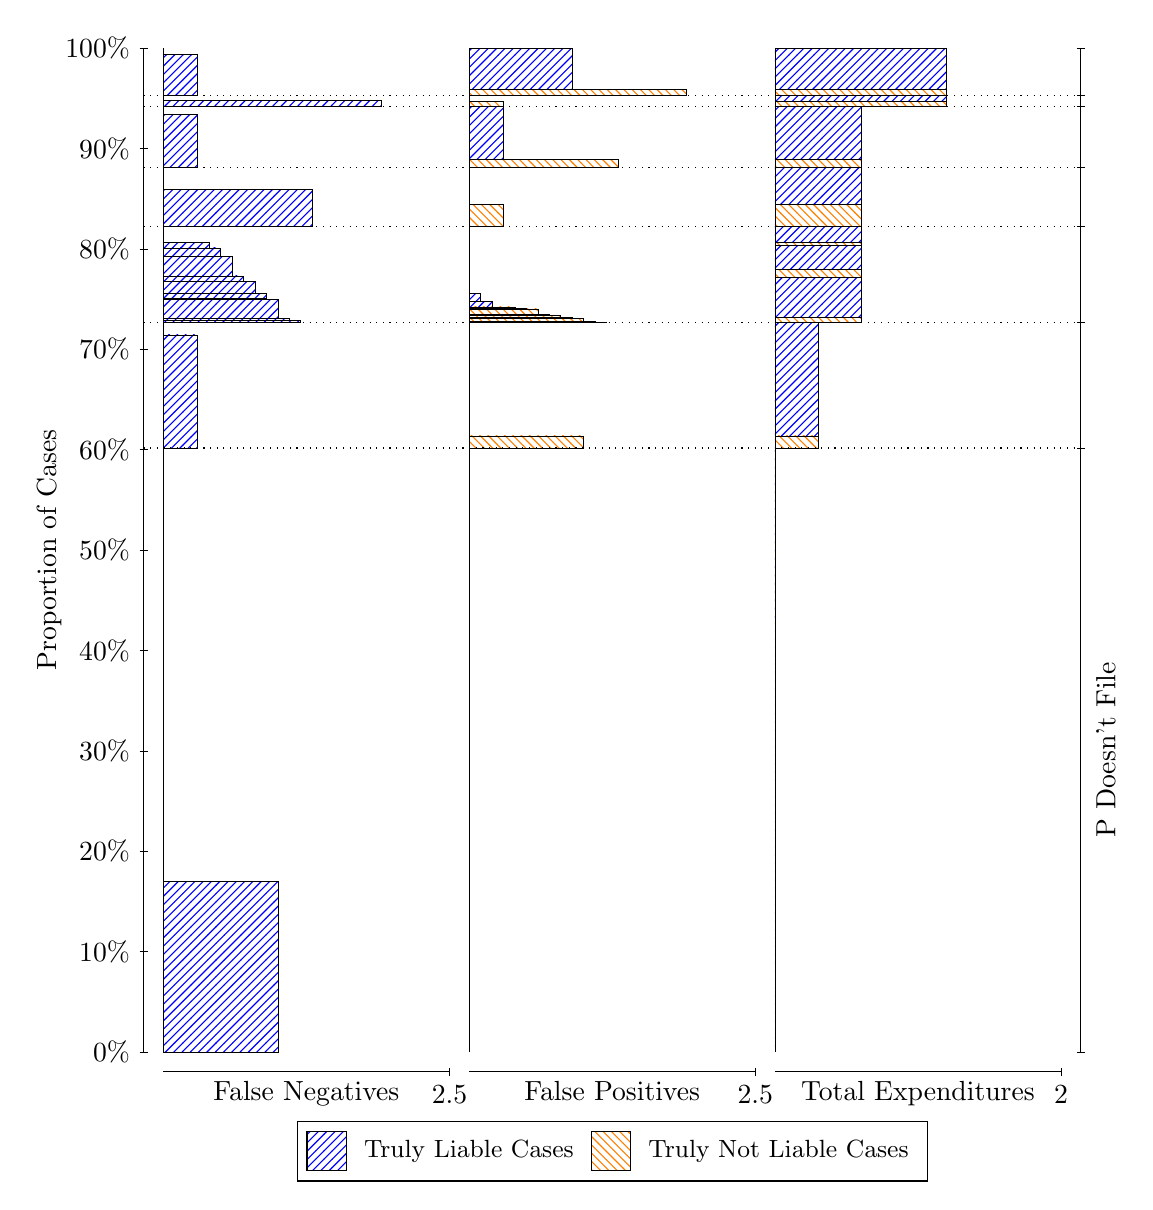
\begin{tikzpicture}
\draw[black, very thin] (1.5,1.75) -- (1.5,14.5);
\node[rotate=90, text=black, anchor=center] at (0.3, 8.125) {Proportion of Cases};
\draw[black, very thin] (1.45,1.75) -- (1.55,1.75);
\node[text=black, anchor=east] at (1.45, 1.75) {0\%};
\draw[black, very thin] (1.45,3.025) -- (1.55,3.025);
\node[text=black, anchor=east] at (1.45, 3.025) {10\%};
\draw[black, very thin] (1.45,4.3) -- (1.55,4.3);
\node[text=black, anchor=east] at (1.45, 4.3) {20\%};
\draw[black, very thin] (1.45,5.575) -- (1.55,5.575);
\node[text=black, anchor=east] at (1.45, 5.575) {30\%};
\draw[black, very thin] (1.45,6.85) -- (1.55,6.85);
\node[text=black, anchor=east] at (1.45, 6.85) {40\%};
\draw[black, very thin] (1.45,8.125) -- (1.55,8.125);
\node[text=black, anchor=east] at (1.45, 8.125) {50\%};
\draw[black, very thin] (1.45,9.4) -- (1.55,9.4);
\node[text=black, anchor=east] at (1.45, 9.4) {60\%};
\draw[black, very thin] (1.45,10.675) -- (1.55,10.675);
\node[text=black, anchor=east] at (1.45, 10.675) {70\%};
\draw[black, very thin] (1.45,11.95) -- (1.55,11.95);
\node[text=black, anchor=east] at (1.45, 11.95) {80\%};
\draw[black, very thin] (1.45,13.225) -- (1.55,13.225);
\node[text=black, anchor=east] at (1.45, 13.225) {90\%};
\draw[black, very thin] (1.45,14.5) -- (1.55,14.5);
\node[text=black, anchor=east] at (1.45, 14.5) {100\%};

\draw[black, very thin] (13.4,1.75) -- (13.4,14.5);
\draw[black, very thin] (13.35,1.75) -- (13.45,1.75);
\node[anchor=west] at (13.35, 1.75) {};
\draw[black, very thin] (13.35,9.4198) -- (13.45,9.4198);
\node[anchor=west] at (13.35, 9.4198) {};
\draw[black, very thin] (13.35,11.012) -- (13.45,11.012);
\node[anchor=west] at (13.35, 11.012) {};
\draw[black, very thin] (13.35,12.231) -- (13.45,12.231);
\node[anchor=west] at (13.35, 12.231) {};
\draw[black, very thin] (13.35,12.986) -- (13.45,12.986);
\node[anchor=west] at (13.35, 12.986) {};
\draw[black, very thin] (13.35,13.76) -- (13.45,13.76);
\node[anchor=west] at (13.35, 13.76) {};
\draw[black, very thin] (13.35,13.898) -- (13.45,13.898);
\node[anchor=west] at (13.35, 13.898) {};
\draw[black, very thin] (13.35,14.5) -- (13.45,14.5);
\node[anchor=west] at (13.35, 14.5) {};

\draw[black, very thin, pattern color=blue, pattern=north east lines] (1.75,1.75) rectangle (3.2033,3.9191);
\draw[black, very thin, pattern color=orange, pattern=north west lines] (1.75,3.9191) rectangle (1.75,9.4198);
\draw[black, very thin, pattern color=blue, pattern=north east lines] (1.75,9.4198) rectangle (2.186,10.858);
\draw[black, very thin, pattern color=orange, pattern=north west lines] (1.75,10.858) rectangle (1.75,11.012);
\draw[black, very thin, pattern color=blue, pattern=north east lines] (1.75,11.012) rectangle (3.494,11.041);
\draw[black, very thin, pattern color=blue, pattern=north east lines] (1.75,11.041) rectangle (3.3487,11.068);
\draw[black, very thin, pattern color=blue, pattern=north east lines] (1.75,11.068) rectangle (3.2033,11.308);
\draw[black, very thin, pattern color=blue, pattern=north east lines] (1.75,11.308) rectangle (3.058,11.324);
\draw[black, very thin, pattern color=blue, pattern=north east lines] (1.75,11.324) rectangle (3.058,11.386);
\draw[black, very thin, pattern color=blue, pattern=north east lines] (1.75,11.386) rectangle (2.9127,11.536);
\draw[black, very thin, pattern color=blue, pattern=north east lines] (1.75,11.536) rectangle (2.7673,11.607);
\draw[black, very thin, pattern color=blue, pattern=north east lines] (1.75,11.607) rectangle (2.622,11.856);
\draw[black, very thin, pattern color=blue, pattern=north east lines] (1.75,11.856) rectangle (2.4767,11.962);
\draw[black, very thin, pattern color=blue, pattern=north east lines] (1.75,11.962) rectangle (2.3313,12.03);
\draw[black, very thin, pattern color=orange, pattern=north west lines] (1.75,12.03) rectangle (1.75,12.231);
\draw[black, very thin, pattern color=blue, pattern=north east lines] (1.75,12.231) rectangle (3.6393,12.707);
\draw[black, very thin, pattern color=orange, pattern=north west lines] (1.75,12.707) rectangle (1.75,12.986);
\draw[black, very thin, pattern color=blue, pattern=north east lines] (1.75,12.986) rectangle (2.186,13.66);
\draw[black, very thin, pattern color=orange, pattern=north west lines] (1.75,13.66) rectangle (1.75,13.76);
\draw[black, very thin, pattern color=blue, pattern=north east lines] (1.75,13.76) rectangle (4.5113,13.838);
\draw[black, very thin, pattern color=orange, pattern=north west lines] (1.75,13.838) rectangle (1.75,13.898);
\draw[black, very thin, pattern color=blue, pattern=north east lines] (1.75,13.898) rectangle (2.186,14.419);
\draw[black, very thin, pattern color=orange, pattern=north west lines] (1.75,14.419) rectangle (1.75,14.5);
\draw[black, very thin, pattern color=orange, pattern=north west lines] (5.6333,1.75) rectangle (5.6333,7.2506);
\draw[black, very thin, pattern color=blue, pattern=north east lines] (5.6333,7.2506) rectangle (5.6333,9.4198);
\draw[black, very thin, pattern color=orange, pattern=north west lines] (5.6333,9.4198) rectangle (7.0867,9.574);
\draw[black, very thin, pattern color=blue, pattern=north east lines] (5.6333,9.574) rectangle (5.6333,11.012);
\draw[black, very thin, pattern color=orange, pattern=north west lines] (5.6333,11.012) rectangle (7.3773,11.019);
\draw[black, very thin, pattern color=orange, pattern=north west lines] (5.6333,11.019) rectangle (7.232,11.033);
\draw[black, very thin, pattern color=orange, pattern=north west lines] (5.6333,11.033) rectangle (7.0867,11.064);
\draw[black, very thin, pattern color=orange, pattern=north west lines] (5.6333,11.064) rectangle (6.9413,11.078);
\draw[black, very thin, pattern color=orange, pattern=north west lines] (5.6333,11.078) rectangle (6.796,11.105);
\draw[black, very thin, pattern color=orange, pattern=north west lines] (5.6333,11.105) rectangle (6.6507,11.12);
\draw[black, very thin, pattern color=orange, pattern=north west lines] (5.6333,11.12) rectangle (6.5053,11.187);
\draw[black, very thin, pattern color=orange, pattern=north west lines] (5.6333,11.187) rectangle (6.36,11.194);
\draw[black, very thin, pattern color=orange, pattern=north west lines] (5.6333,11.194) rectangle (6.2147,11.213);
\draw[black, very thin, pattern color=blue, pattern=north east lines] (5.6333,11.213) rectangle (5.924,11.281);
\draw[black, very thin, pattern color=blue, pattern=north east lines] (5.6333,11.281) rectangle (5.7787,11.388);
\draw[black, very thin, pattern color=blue, pattern=north east lines] (5.6333,11.388) rectangle (5.6333,12.231);
\draw[black, very thin, pattern color=orange, pattern=north west lines] (5.6333,12.231) rectangle (6.0693,12.51);
\draw[black, very thin, pattern color=blue, pattern=north east lines] (5.6333,12.51) rectangle (5.6333,12.986);
\draw[black, very thin, pattern color=orange, pattern=north west lines] (5.6333,12.986) rectangle (7.5227,13.086);
\draw[black, very thin, pattern color=blue, pattern=north east lines] (5.6333,13.086) rectangle (6.0693,13.76);
\draw[black, very thin, pattern color=orange, pattern=north west lines] (5.6333,13.76) rectangle (6.0693,13.819);
\draw[black, very thin, pattern color=blue, pattern=north east lines] (5.6333,13.819) rectangle (5.6333,13.898);
\draw[black, very thin, pattern color=orange, pattern=north west lines] (5.6333,13.898) rectangle (8.3947,13.978);
\draw[black, very thin, pattern color=blue, pattern=north east lines] (5.6333,13.978) rectangle (6.9413,14.5);
\draw[black, very thin, pattern color=orange, pattern=north west lines] (9.5167,1.75) rectangle (9.5167,7.2506);
\draw[black, very thin, pattern color=blue, pattern=north east lines] (9.5167,7.2506) rectangle (9.5167,9.4198);
\draw[black, very thin, pattern color=orange, pattern=north west lines] (9.5167,9.4198) rectangle (10.062,9.574);
\draw[black, very thin, pattern color=blue, pattern=north east lines] (9.5167,9.574) rectangle (10.062,11.012);
\draw[black, very thin, pattern color=orange, pattern=north west lines] (9.5167,11.012) rectangle (10.607,11.084);
\draw[black, very thin, pattern color=blue, pattern=north east lines] (9.5167,11.084) rectangle (10.607,11.589);
\draw[black, very thin, pattern color=orange, pattern=north west lines] (9.5167,11.589) rectangle (10.607,11.685);
\draw[black, very thin, pattern color=blue, pattern=north east lines] (9.5167,11.685) rectangle (10.607,11.998);
\draw[black, very thin, pattern color=orange, pattern=north west lines] (9.5167,11.998) rectangle (10.607,12.031);
\draw[black, very thin, pattern color=blue, pattern=north east lines] (9.5167,12.031) rectangle (10.607,12.231);
\draw[black, very thin, pattern color=orange, pattern=north west lines] (9.5167,12.231) rectangle (10.607,12.51);
\draw[black, very thin, pattern color=blue, pattern=north east lines] (9.5167,12.51) rectangle (10.607,12.986);
\draw[black, very thin, pattern color=orange, pattern=north west lines] (9.5167,12.986) rectangle (10.607,13.086);
\draw[black, very thin, pattern color=blue, pattern=north east lines] (9.5167,13.086) rectangle (10.607,13.76);
\draw[black, very thin, pattern color=orange, pattern=north west lines] (9.5167,13.76) rectangle (11.697,13.819);
\draw[black, very thin, pattern color=blue, pattern=north east lines] (9.5167,13.819) rectangle (11.697,13.898);
\draw[black, very thin, pattern color=orange, pattern=north west lines] (9.5167,13.898) rectangle (11.697,13.978);
\draw[black, very thin, pattern color=blue, pattern=north east lines] (9.5167,13.978) rectangle (11.697,14.5);
\draw[black, dotted] (1.5,9.4198) -- (13.4,9.4198);
\draw[black, dotted] (1.5,11.012) -- (13.4,11.012);
\draw[black, dotted] (1.5,12.231) -- (13.4,12.231);
\draw[black, dotted] (1.5,12.986) -- (13.4,12.986);
\draw[black, dotted] (1.5,13.76) -- (13.4,13.76);
\draw[black, dotted] (1.5,13.898) -- (13.4,13.898);
\draw[black, very thin] (1.75,1.5) -- (5.3833,1.5);
\node[text=black, anchor=north] at (3.5667, 1.5) {False Negatives};
\draw[black, very thin] (5.3833,1.45) -- (5.3833,1.55);
\node[text=black, anchor=north] at (5.3833, 1.45) {2.5};

\draw[black, very thin] (5.6333,1.5) -- (9.2667,1.5);
\node[text=black, anchor=north] at (7.45, 1.5) {False Positives};
\draw[black, very thin] (9.2667,1.45) -- (9.2667,1.55);
\node[text=black, anchor=north] at (9.2667, 1.45) {2.5};

\draw[black, very thin] (9.5167,1.5) -- (13.15,1.5);
\node[text=black, anchor=north] at (11.333, 1.5) {Total Expenditures};
\draw[black, very thin] (13.15,1.45) -- (13.15,1.55);
\node[text=black, anchor=north] at (13.15, 1.45) {2};

\node[text=black, centered, rotate=90] at (13.72, 5.5849) {P Doesn't File};







\draw (7.449999999999999,1.5) node[draw=none] (baseCoordinate) {};
\begin{scope}[align=center]
        \matrix[scale=0.5, draw=black, below=0.5cm of baseCoordinate, nodes={draw}, column sep=0.1cm]{
            \node[rectangle, draw, minimum width=0.5cm, minimum height=0.5cm, pattern color=blue, pattern=north east lines] {}; &
            \node[draw=none, font=\small, text=black] (B) {Truly Liable Cases}; &
            \node[rectangle, draw, minimum width=0.5cm, minimum height=0.5cm, pattern color=orange, pattern=north west lines] {}; &
            \node[draw=none, font=\small, text=black] (B) {Truly Not Liable Cases}; \\
            };
\end{scope}

\end{tikzpicture}
\end{document}